\documentclass[]{article}
\usepackage[all]{xy}
\usepackage{amsmath}
\usepackage{amssymb}
\usepackage{amsthm}
\usepackage{indentfirst}
\usepackage{listings}
\usepackage{multirow}
\usepackage{tikz}
\usepackage{tikz-qtree}
\usepackage{tipa}
\usetikzlibrary{arrows,automata}
\begin{document}

\newtheorem{thm}{Theorem}

\title{COMS W3261 \\ Computer Science Theory \\ Homework \#1}
\author{Alexander Roth}
\date{2014 -- 09 -- 15}
\maketitle

\section*{Problems}
  \begin{enumerate}
    \item Use a computer program that supports regular expressions to find the 
    lexicographically first longest English word in the dictionary that can be
    made up using only letters in your first and last name. A letter in your 
    name can be used zero or more times. Show the regular expression and program
    you used to find your answer.
    \item[\emph{Solution}] My name is Alexander Roth. After removing duplicate
    characters, we are left with the string \texttt{alexndroth}. Now, it must
    be a string that solely contains these characters; thus, we capture these
    characters with \texttt{[} and \texttt{]}, like so \texttt{[alexndroth]}.
    Now, since these strings cannot be substrings of other words, we must 
    include \texttt{\^{}} to signify the beginning of the string, and 
    \texttt{\$} to signify the end of the string. To find all matches, we would 
    include \texttt{*} as the operator, which gives a large list of words when 
    passed into egreps. Thus, our regular expression passed into egrep is: \\\\
      \texttt{egrep `\^{}[alexndroth]*\$' /usr/share/dict/words} \\\\
    which prints three words of length 15, the first being ``hexatetrahedron''. 
    I found the longest first string by using a small program I wrote 
    (shown below).
    
    \lstinputlisting[language=Python]{../length_check.py} 
    \item In Lecture 2 (September 8, 2014) we presented a three-state DFA that
    recognizes exactly those binary strings representing integers divisible by 
    3. Using induction, prove that state A represents all and only the prefixes 
    of binary strings that are numbers congruent to 0 mod 3, state B all and 
    only the prefixes congruent to 1 mod 3, and state C all and only the 
    prefixes congruent to 2 mod 3

    \item[\emph{Solution}]
           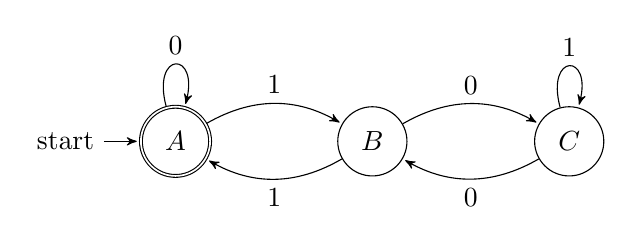
\begin{tikzpicture}[>=stealth',shorten >=1pt,auto,node 
          distance=2.5cm]
        \node[initial,state,accepting] (A)              {$A$};
        \node[state]                   (B) [right of=A] {$B$};
        \node[state]                   (C) [right of=B] {$C$};
        \path[->] (A) edge [loop above] node {0} (A);
        \path[->] (A) edge [bend left]  node {1} (B);
        \path[->] (B) edge [bend left]  node {1} (A);
        \path[->] (B) edge [bend left]  node {0} (C);
        \path[->] (C) edge [bend left]  node {0} (B);
        \path[->] (C) edge [loop above] node {1} (C);
      \end{tikzpicture} 
      \begin{itemize}
        \item Consider the DFA $D = (\{A,B,C\}, \{0,1\}, \delta, A, \{A\})$ 
        where the transition function $\delta$ has the transition diagram shown
        above.
        \item Let $L$ be the language consisting of all binary strings 
        representing integers divisible by 3. We shall prove that $L(D) = L$.
        \item To begin, we shall show that every string accepted by $D$ is in $L
        $, by proving the following inductive hypothesis by induction on $n$, 
        the moves made by $D$ accepting a binary string $w$, for $n \geq 0$:
        \\ Inductive Hypothesis 1:
          \begin{enumerate}
            \item If $\delta^n(A,w) = A$, then $w$ is a binary string whose 
            value is equivalent to 0 mod 3. Here $\delta^n$ means $n$ moves by 
            $D$.
            \item If $\delta^n(B,w) = B$, then $w$ is a binary string whose 
            value is equivalent to 1 mod 3.
            \item If $\delta^n(C,w) = C$, then $w$ is a binary string whose 
            value is equivalent to 2 mod 3.
              \begin{itemize}
                \item Basis. $n = 0$ which implies that $w = \epsilon$ Note that 
                by appending a $1$ to $w$, the value of $w$ is $2x + 1$, where 
                $x$ is the original string. Similarly, appending $0$ to $w$ 
                gives us the value $2x$ where $x$ is the substring without $0$.
                \item Induction. Assume that IH1 is true for 
                $0, 1, 2, \ldots, n$ moves.
                  \begin{itemize}
                    \item Suppose $D$ makes $n + 1$ moves on a string $w = x1$ 
                    and enters state $A$ after reading $x$ and then enters state 
                    $B$ after reading the final $1$. The value of $w$ is $2x + 
                    1$. From the inductive hypothesis, we know that $x$ must be 
                    a binary string with a value congruent to 0 mod 3. 
                    Therefore, $x1$ must be a binary string congruent to 1 mod 
                    3.
                    \item Suppose $D$ makes $n + 1$ moves on a string $w = x0$ 
                    and enters state $A$ after reading $x$ and then enters state
                    $A$ after reading the final $0$. The value of $w$ is 2x. 
                    From the inductive hypothesis, we know that $x$ must be a 
                    binary string with a value congruent to 0 mod 3. Therefore, 
                    $x0$ must also be a binary string congruent to 0 mod 3.
                    \item Suppose $D$ makes $n + 1$ moves on a string $w = x1$ 
                    and enters state $B$ after reading $x$ and then enters state 
                    $A$ after reading the final $1$. The value of $w$ is $2x + 
                    1$, From the inductive hypothesis, we know that $x$ must be 
                    a binary string with a value congruent to 1 mod 3. Thus, 
                    $x1$ must be a binary string congruent to 0 mod 3.
                    \item Suppose $D$ makes $n + 1$ moves on a string $w = x0$ 
                    and enters state $B$ after reading $x$ and then enters state 
                    $C$ after reading the final $0$. The value of $w$ is $2x$. 
                    From the inductive hypothesis, we know that $x$ must be a 
                    binary string with a value congruent to 1 mod 3. Therefore, 
                    $x1$ must be a binary string congruent to 2 mod 3.
                    \item Suppose $D$ makes $n + 1$ moves on a string $w = x1$ 
                    and enters state $C$ after reading $x$ and then enters state 
                    $C$ after reading the final $1$. The value of $w$ is $2x + 
                    1$. From the inductive hypothesis, we know that $x$ must be 
                    a binary string with a value congruent to 2 mod 3. 
                    Therefore, $x1$ must also be a binary string congruent to 2 
                    mod 3.
                    \item Suppose $D$ makes $n + 1$ moves on a string $w = x0$
                    and enters state $C$ after reading $x$ and the enters state 
                    $B$ after reading the final $0$. The value of $w$ is $2x$. 
                    From the inductive hypothesis, we know that $x$ must be a 
                    binary string a value congruent to 2 mod 3. Therefore, $x0$ 
                    must be a binary string congruent to 1 mod 3.
                  \end{itemize}
              \end{itemize}
          \end{enumerate}
        \item We have now shown that IH1 is true for all sequences of $n$ 
        moves, where $n \geq 0$.
        \item We now need to show that every string in $L$ is accepted by $D$. 
        To do this, we shall prove the following inductive hypothesis by 
        induction on $n$, the length of a string $w$ for $n \geq 0$: \\
        Inductive Hypothesis IH2:
          \begin{enumerate}
            \item If $w$ is a binary string that has a value congruent to 0 mod 
            3, then $\delta^*(A,w) = A$. 
            \item If $w$ is a binary string that has a value congruent to 1 mod 
            3, then $\delta^*(B,w) = B$.
            \item If $w$ is a binary string that has a value congruent to 2 mod
            3, then $\delta^*(C,w) = C$.
              \begin{itemize}
                \item Basis. $n = 0$; that is $w = \epsilon$. $D$ accepts the 
                empty string since the start state is a final state.
                \item Induction. Assume IH2 is true for all string $w$ of length 
                $0,1,2,\ldots,n$.
                  \begin{itemize}
                    \item Suppose $w$ is now a string of length $n + 1$ and 
                    $w = x0$ and $x$ is a binary string that has a value 
                    congruent to 0 mod 3. From IH2, $\delta^*(A,x)=A$. Since 
                    $\delta(A,0)=A$, $\delta^*(A,w)=A$. That is, the value of $w
                    $ is $2x$, which is equivalent to 0 mod 3.
                    \item Suppose $w$ is now a string of length $n + 1$ and 
                    $w = x1$ and $x$ is a binary string that has a value 
                    congruent to 0 mod 3. From IH2, $\delta^*(A,x)=A$. Since 
                    $\delta(A,1)=B$, $\delta^*(A,w)=B$. That is, the value of $w
                    $ is $2x + 1$, which is equivalent to 1 mod 3.
                    \item Suppose $w$ is now a string of length $n + 1$ and
                    $w = x0$ and $x$ is a binary string that has a value 
                    congruent to 1 mod 3. From IH2, $\delta^*(B,x)=B$. Since 
                    $\delta(B,0)=C$, $\delta^*(B,w)=C$. That is, $w$ has a value 
                    of $2x$, which is equivalent to 2 mod 3.
                    \item Suppose $w$ is now a string of length $n + 1$ and
                    $w = x1$ and $x$ is a binary string that has a value 
                    congruent to 1 mod 3. From IH2, $\delta^*(B,x)=B$. Since 
                    $\delta(B,1)=A$, $\delta^*(B,w)=A$. That is, $w$ has a value 
                    of $2x + 1$, which is equivalent to 0 mod 3.
                    \item Suppose $w$ is now a string of length $n + 1$ and
                    $w = x0$ and $x$ is a binary string that has a value 
                    congruent to 2 mod 3. From IH2, $\delta^*(C,x)=C$. Since 
                    $\delta(C,0)=B$, $\delta^*(C,w)=B$. That is, $w$ has a value 
                    of $2x$, which is equivalent to 1 mod 3
                    \item Suppose $w$ is now a string of length $n + 1$ and 
                    $w = x1$ and $x$ is a binary string that has a value 
                    congruent to 2 mod 3. From IH2, $\delta^*(C,x)=C$. Since
                    $\delta(C,1)=C$, $\delta^*(C,w)=C$. That is, $w$ has a value
                    of $2x + 1$, which is equivalent to 2 mod 3.
                  \end{itemize}
              \end{itemize}
          \end{enumerate}
        \item We have now shown that IH2 is true for all strings of length $n$, 
        $n \geq 0$.
        \item From the two inductive hypotheses, we can conclude that $w$ is 
        accepted by $D$ iff $w$ is in $L$. In other words, $L(D) = L$.
      \end{itemize}
    \newpage
    \item Let $L$ be the language generated by the regular expression 
      \[ (a+b)^*a(a+b)(a+b) \]
      \begin{enumerate}
        \item Construct a nondeterministic finite automaton (NFA) for $L$. 
        (Identify the five components of your NFA. Use a transition diagram for 
        the transition function.)
        \item Show how your NFA processes the input string \texttt{abaab}.
        \item Using the subset construction convert your NFA into an equivalent 
        DFA.
        \item Show how your DFA processes the input string \texttt{abaab}.
      \end{enumerate}
      \item[\emph{Solution}]
      \begin{enumerate}
        \item The five components are:
          \[  
            A = (\{q_0, q_1, q_2, q_3 \}, 
                 \{\texttt{a}, \texttt{b}\}, 
                 \delta, 
                 q_0,
                 q_3)
          \]
          where $\delta$ is the transition diagram represented below. \\
          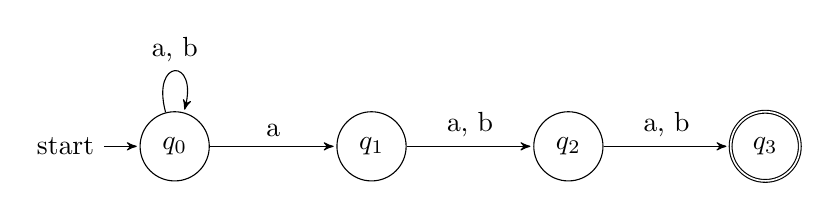
\begin{tikzpicture}[>=stealth',shorten >=1pt,auto,node distance=2.5cm]
            \node[initial, state]  (q_0)                {$q_0$};
            \node[state]           (q_1) [right of=q_0] {$q_1$};
            \node[state]           (q_2) [right of=q_1] {$q_2$};
            \node[state,accepting] (q_3) [right of=q_2] {$q_3$};  
            \path[->] (q_0) edge [loop above] node {a, b} (q_0);
            \path[->] (q_0) edge              node {a}    (q_1);
            \path[->] (q_1) edge              node {a, b} (q_2);
            \path[->] (q_2) edge              node {a, b} (q_3);
          \end{tikzpicture}
        \item
          \begin{displaymath}
            \xymatrix{q_0 \ar[r]^a \ar[dr]^a & q_0 \ar[r]^b  & q_0 \ar[r]^a \ar[dr]^a & q_0 \ar[r]^a \ar[dr]^a  & q_0 \ar[r]^b  & q_0 \\
                                             & q_1 \ar[dr]^b &                        & q_1 \ar[dr]^a           & q_1 \ar[dr]^b &     \\
                                             &               & q_2 \ar[dr]^a          &                         & q_2 \ar[dr]^b & q_2 \\ 
                                             &               &                        & q_3                     &               & q_3 }
          \end{displaymath} 
          where the initial $q_3$ becomes stuck, due to its inability to 
          process the rest of the string.
        \item We have this transition table formed through ``lazy evaluation'': 
        \\
          \begin{tabular}{c|c|c}
                                  & a                  & b             \\ \hline
            $\rightarrow \{q_0\}$ & $\{q_0, q_1\}$     & $\{q_0\}$     \\
            $\{q_0, q_1\}$        & $\{q_0,q_1,q_2\}$  & $\{q_0,q_2\}$ \\
            $\{q_0, q_2\}$        & $\{q_0,q_1,q_3\}$  & $\{q_0,q_3\}$ \\
            $*\{q_0, q_3\}$       & $\{q_0,q_1\}$      & $\{q_0\}$     \\
            $\{q_0,q_1,q_2\}$     & $\{q_0,q_1,q_2,q_3\}$ & $\{q_0,q_2,q_3\}$ \\
            $*\{q_0,q_1,q_3\}$    & $\{q_0,q_1,q_2\}$ & $\{q_0,q_2\}$ \\
            $*\{q_0,q_2,q_3\}$    & $\{q_0,q_1,q_3\}$ & $\{q_0,q_3\}$ \\
            $*\{q_0,q_1,q_2,q_3\}$& $\{q_0,q_1,q_2,q_3\}$ & $\{q_0,q_2,q_3\}$
          \end{tabular} \\ 
        Let us rename the transition state table using states $A, \ldots$ \\
          \begin{tabular}{c|c|c}
                            & a   & b   \\ \hline
            $\rightarrow A$ & $B$ & $A$ \\
            $B$             & $E$ & $C$ \\
            $C$             & $F$ & $D$ \\
            $*D$            & $B$ & $A$ \\
            $E$             & $H$ & $G$ \\
            $*F$            & $E$ & $C$ \\
            $*G$            & $F$ & $D$ \\
            $*H$            & $H$ & $G$ \\
          \end{tabular} \\
        which gives us the transition diagram: \\
          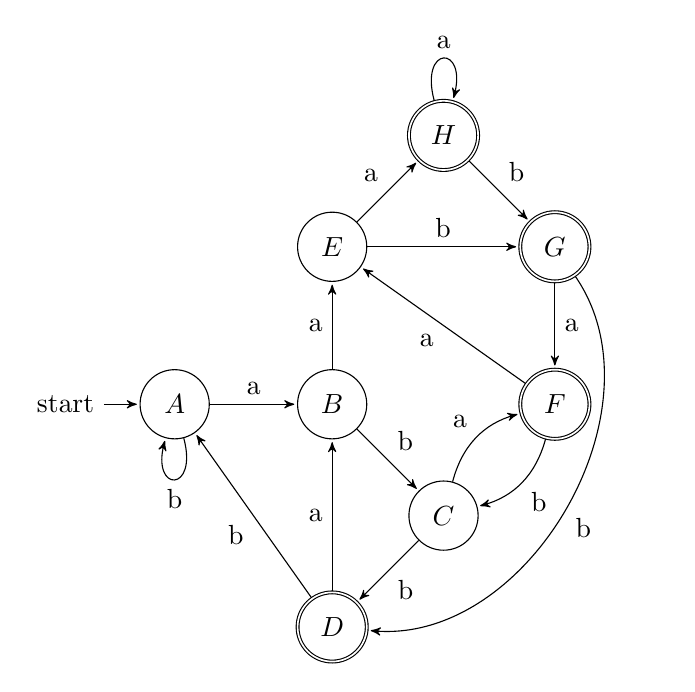
\begin{tikzpicture}[->,>=stealth',shorten >=1pt,auto,node 
            distance=2cm]
            \node[initial, state]  (A)                    {$A$};
            \node[state]           (B) [right of=A]       {$B$};
            \node[state]           (E) [above of=B]       {$E$};
            \node[state]           (C) [below right of=B] {$C$};
            \node[state,accepting] (D) [below left of=C]  {$D$};
            \node[state,accepting] (H) [above right of=E] {$H$};
            \node[state,accepting] (G) [below right of=H] {$G$};
            \node[state,accepting] (F) [below of=G]       {$F$};
            \path[->] (A) edge [loop below]   node {b} (A);
            \path[->] (A) edge                node {a} (B);
            \path[->] (B) edge                node {a} (E);
            \path[->] (B) edge                node {b} (C);
            \path[->] (C) edge                node {b} (D);
            \path[->] (D) edge                node {a} (B);
            \path[->] (D) edge                node {b} (A);
            \path[->] (C) edge [bend left]    node {a} (F);
            \path[->] (F) edge [bend left]    node {b} (C);
            \path[->] (F) edge                node {a} (E);
            \path[->] (E) edge                node {b} (G);
            \path[->] (G) edge                node {a} (F);
            \path[->] (G) edge [bend left=65] node {b} (D);
            \path[->] (E) edge                node {a} (H);
            \path[->] (H) edge [loop above]   node {a} (H);
            \path[->] (H) edge                node {b} (G);

          \end{tikzpicture} \\
        So now that we have this monstrosity, we have 
          \[ A = (Q, \Sigma, \delta, q_0, F) \]
        where 
          \begin{enumerate}
            \item[1.] $Q = \{ A, B, E, F, G, H\}$
            \item[2.] $\Sigma = \{a, b\}$
            \item[3.] $\delta$ is the transition diagram pictured above.
            \item[4.] $q_0$ is state $A$.
            \item[5.] $F = \{D, F, G, H\}$.
          \end{enumerate} 
        \item We start on state $A$. The machine reads an $a$ and transitions to 
        state $B$, we then read a $b$, and move to state $C$. From there, we 
        read an $a$ and move to state $F$. The machine reads another $a$ and 
        moves to state $E$. Finally, the machine reads the last character, a $b$
        and halts on state $G$, accepting the string $abaab$.
      \end{enumerate}  
    \item Construct an epsilon-NFA from the regular expression in problem (3) 
    using the McNaughton-Yamada-Thompson algorithm. Show how your epsilon-NFA 
    processes the input string \texttt{abaab}.
    \item[\emph{Solution}] The regular expression in (3) is 
      \[ (a + b)^*a(a + b)(a + b) \]
    Our $\epsilon$-NFA is shown on the next page: \\
      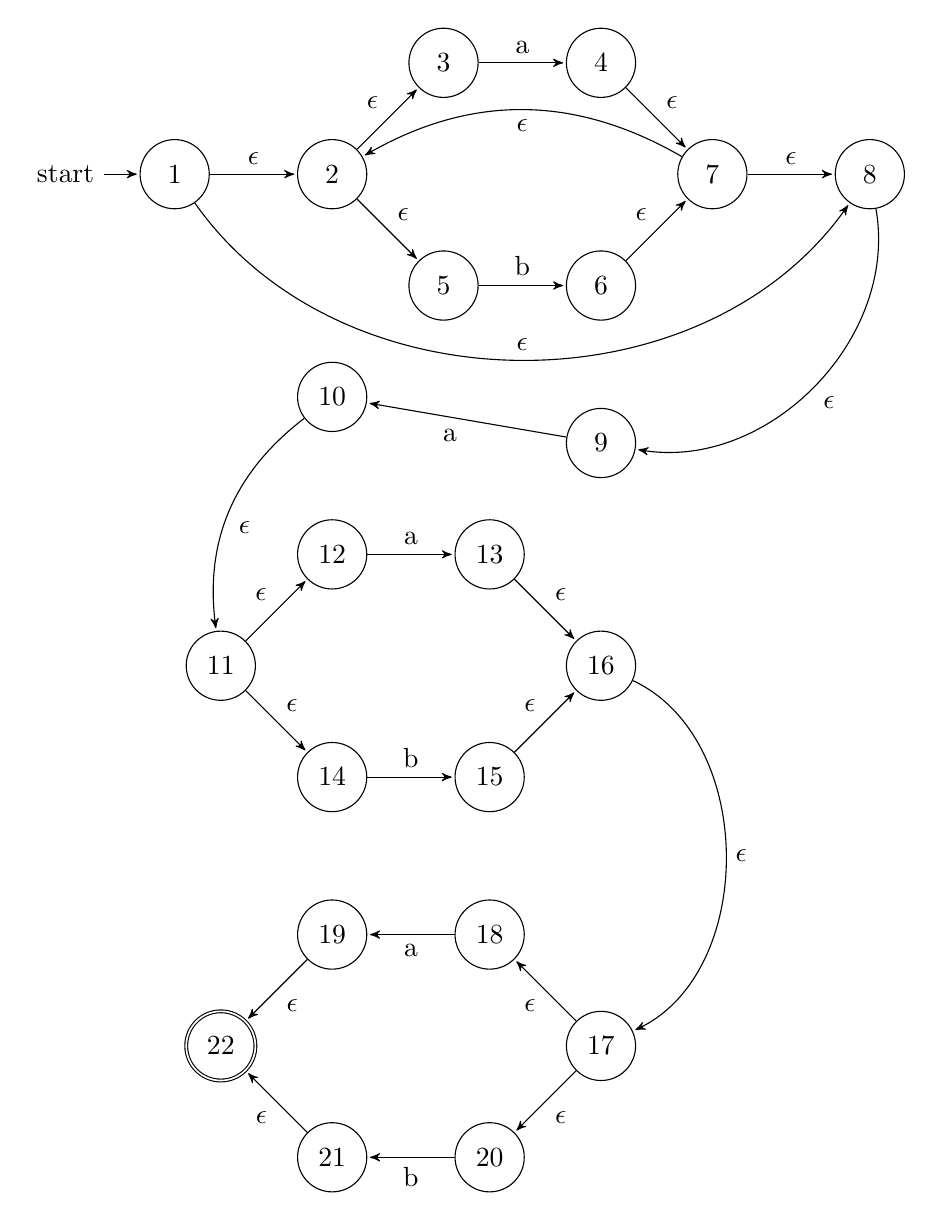
\begin{tikzpicture}[->,>=stealth',shorten >=1pt,auto,node distance=2cm]
        \node[state,initial]   (1)                      {$1$};
        \node[state]           (2)  [right of=1]        {$2$};
        \node[state]           (3)  [above right of=2]  {$3$};
        \node[state]           (4)  [right of=3]        {$4$};
        \node[state]           (5)  [below right of=2]  {$5$};
        \node[state]           (6)  [right of=5]        {$6$};
        \node[state]           (7)  [below right of=4]  {$7$};
        \node[state]           (8)  [right of=7]        {$8$};
        \node[state]           (9)  [below of=6]        {$9$};
        \node[state]           (10) [below left of=5]   {$10$};
        \node[state]           (12) [below of=10]       {$12$};
        \node[state]           (11) [below left of=12]  {$11$};
        \node[state]           (13) [right of=12]       {$13$};
        \node[state]           (14) [below right of=11] {$14$};
        \node[state]           (15) [right of=14]       {$15$};
        \node[state]           (16) [below right of=13] {$16$};
        \node[state]           (19) [below of=14]       {$19$};
        \node[state]           (18) [below of=15]       {$18$};
        \node[state]           (17) [below right of=18] {$17$};
        \node[state,accepting] (22) [below left of=19]  {$22$};
        \node[state]           (20) [below left of=17]  {$20$};
        \node[state]           (21) [left of=20]        {$21$};
        \path[->] (1)  edge                 node {$\epsilon$} (2);
        \path[->] (2)  edge                 node {$\epsilon$} (3);
        \path[->] (3)  edge                 node {a}          (4);
        \path[->] (2)  edge                 node {$\epsilon$} (5);
        \path[->] (5)  edge                 node {b}          (6);
        \path[->] (4)  edge                 node {$\epsilon$} (7);
        \path[->] (6)  edge                 node {$\epsilon$} (7);
        \path[->] (7)  edge                 node {$\epsilon$} (8);
        \path[->] (1)  edge [bend right=55] node {$\epsilon$} (8);
        \path[->] (7)  edge [bend right]    node {$\epsilon$} (2);
        \path[->] (8)  edge [bend left=55]  node {$\epsilon$} (9);
        \path[->] (9)  edge                 node {a}          (10);
        \path[->] (10) edge [bend right]    node {$\epsilon$} (11);
        \path[->] (11) edge                 node {$\epsilon$} (12);
        \path[->] (11) edge                 node {$\epsilon$} (14);
        \path[->] (12) edge                 node {a}          (13);
        \path[->] (14) edge                 node {b}          (15);
        \path[->] (13) edge                 node {$\epsilon$} (16);
        \path[->] (15) edge                 node {$\epsilon$} (16);
        \path[->] (16) edge [bend left=65]  node {$\epsilon$} (17);
        \path[->] (17) edge                 node {$\epsilon$} (18);
        \path[->] (18) edge                 node {a}          (19);
        \path[->] (17) edge                 node {$\epsilon$} (20);
        \path[->] (20) edge                 node {b}          (21);
        \path[->] (19) edge                 node {$\epsilon$} (22);
        \path[->] (21) edge                 node {$\epsilon$} (22);
      \end{tikzpicture} \\
      \begin{tabular}{c|c}
        Possible States                        & Next Input          \\ \hline
        $ \rightarrow \{1,2,3,5,8,9\}$                 & a           \\
        $ \{4,7,2,3,5,8,9,10,11,12,14\}$               & b           \\
        $ \{6,7,2,3,5,8,9,15,16,17,18,20\}$            & a           \\
        $*\{4,7,2,3,5,8,9,10,11,12,14,19,22\}$         & a           \\       
        $\{4,7,2,3,5,8,9,10,11,12,14,13,16,17,18,20\}$ & b           \\
        $*\{6,7,2,3,5,8,9,15,16,17,18,20,21,22\}$     & $\emptyset$ \\
      \end{tabular} \\
     Thus, the string \texttt{abaab} is accepted by this machine. The path is
        \[
           1, 2, 3, 4, 7, 2, 5, 6, 7, 8, 9, 10, 11, 12, 13, 16, 17, 20, 21, 22
        \]
    and this is found by following the epsilon closures after each input
    is read. The string will be accepted by this $\epsilon$-NFA.
    \item Let $L$ be the language $\{ w \, | \, w$ is any string of $a$'s and
    $b$'s where the number of $a$'s is different from the number of $b$'s $\}$.
    If $L$ is regular, construct a DFA for $L$; if not, prove that $L$ is not
    regular.
    \item[\emph{Solution:}] Let us assume that $L$ is a regular language. Then 
    $L = L(A)$ for some DFA $A$. Since $L$ can be represented by a DFA, we can
    suppose that $A$ has $n$ states. Thus, we can apply the pumping lemma to 
    DFA $A$, where $A$ represents $L$, which is the language of any string of 
    $a$'s and $b$'s where the number of $a$'s is different from the number of 
    $b$'s. Using the Closure of Regular Languages under Complementation, we can 
    find a complimentary language $\overline{L} = L(B)$ such that $B$ is a DFA 
    $(Q, \Sigma, \delta, q_0, Q-F)$, that is $B$ is exactly like $A$, but the 
    accepting states of $A$ have become nonaccepting states of $B$. In our case,
    that means the only strings in this language are all strings of equal number
    of $a$'s and $b$'s (not in any particular order). \\ \\
    Now we use the pumping lemma to show that the complimentary language
    of $L$ is not regular, via a proof by contradiction. Since $\overline{L}$ is
    a regular language, as stated above, we can apply the pumping lemma to it.
    Suppose $n$ is the constant that must exist if $\overline{L}$ is regular. We
    then pick a string $w = a^nb^n$, that is, $n$ $a$'s followed by $n$ $b$'s, a
    string with equal $a$'s and $b$'s that must be in $\overline{L}$. Now, the
    string can be broken into three parts: $x$, $y$, and $z$. All we know is
    that $y \neq \epsilon$, and $|xy| \leq n$. Since $|xy| \leq n$, and $xy$
    comes at the front of $W$, we know that $x$ and $y$ only consist of $a$'s. 
    The pumping lemma tells us that $xz$ is in $\overline{L}$, if $\overline{L}$ 
    is regular, when $k = 0$. However, $xz$ has $n$ $b$'s, since all the $b$'s 
    of $w$ are in $z$. But $xz$ also has fewer tha $n$ $a$'s, because we lost 
    the $a$'s of $y$. Since $y \neq \epsilon$, we know that there can be no more 
    than $n - 1$ $a$'s among $x$ and $z$. Thus, after assuming $\overline{L}$ is 
    a regular language, we have proved a fact known to be false, that $xz$ is in 
    $\overline{L}$, which is a clear violation of condition (3) of the pumping 
    lemma. We have a proof by contradiction of the fact that
    $\overline{L}$ is not regular.\\\\
    Using the closure under complementation for Regular Languages, we know that 
    the complement of a regular language is another regular language. Since we 
    proved that $\overline{L}$ is not a regular language, we have also proved 
    that $L$ is not a regular language.
      
  \end{enumerate}

\end{document}